Voici ci-dessous, la structure originale de la machine au commencement de ce projet de Bachelor :
\begin{figure}[H]
  \centering
  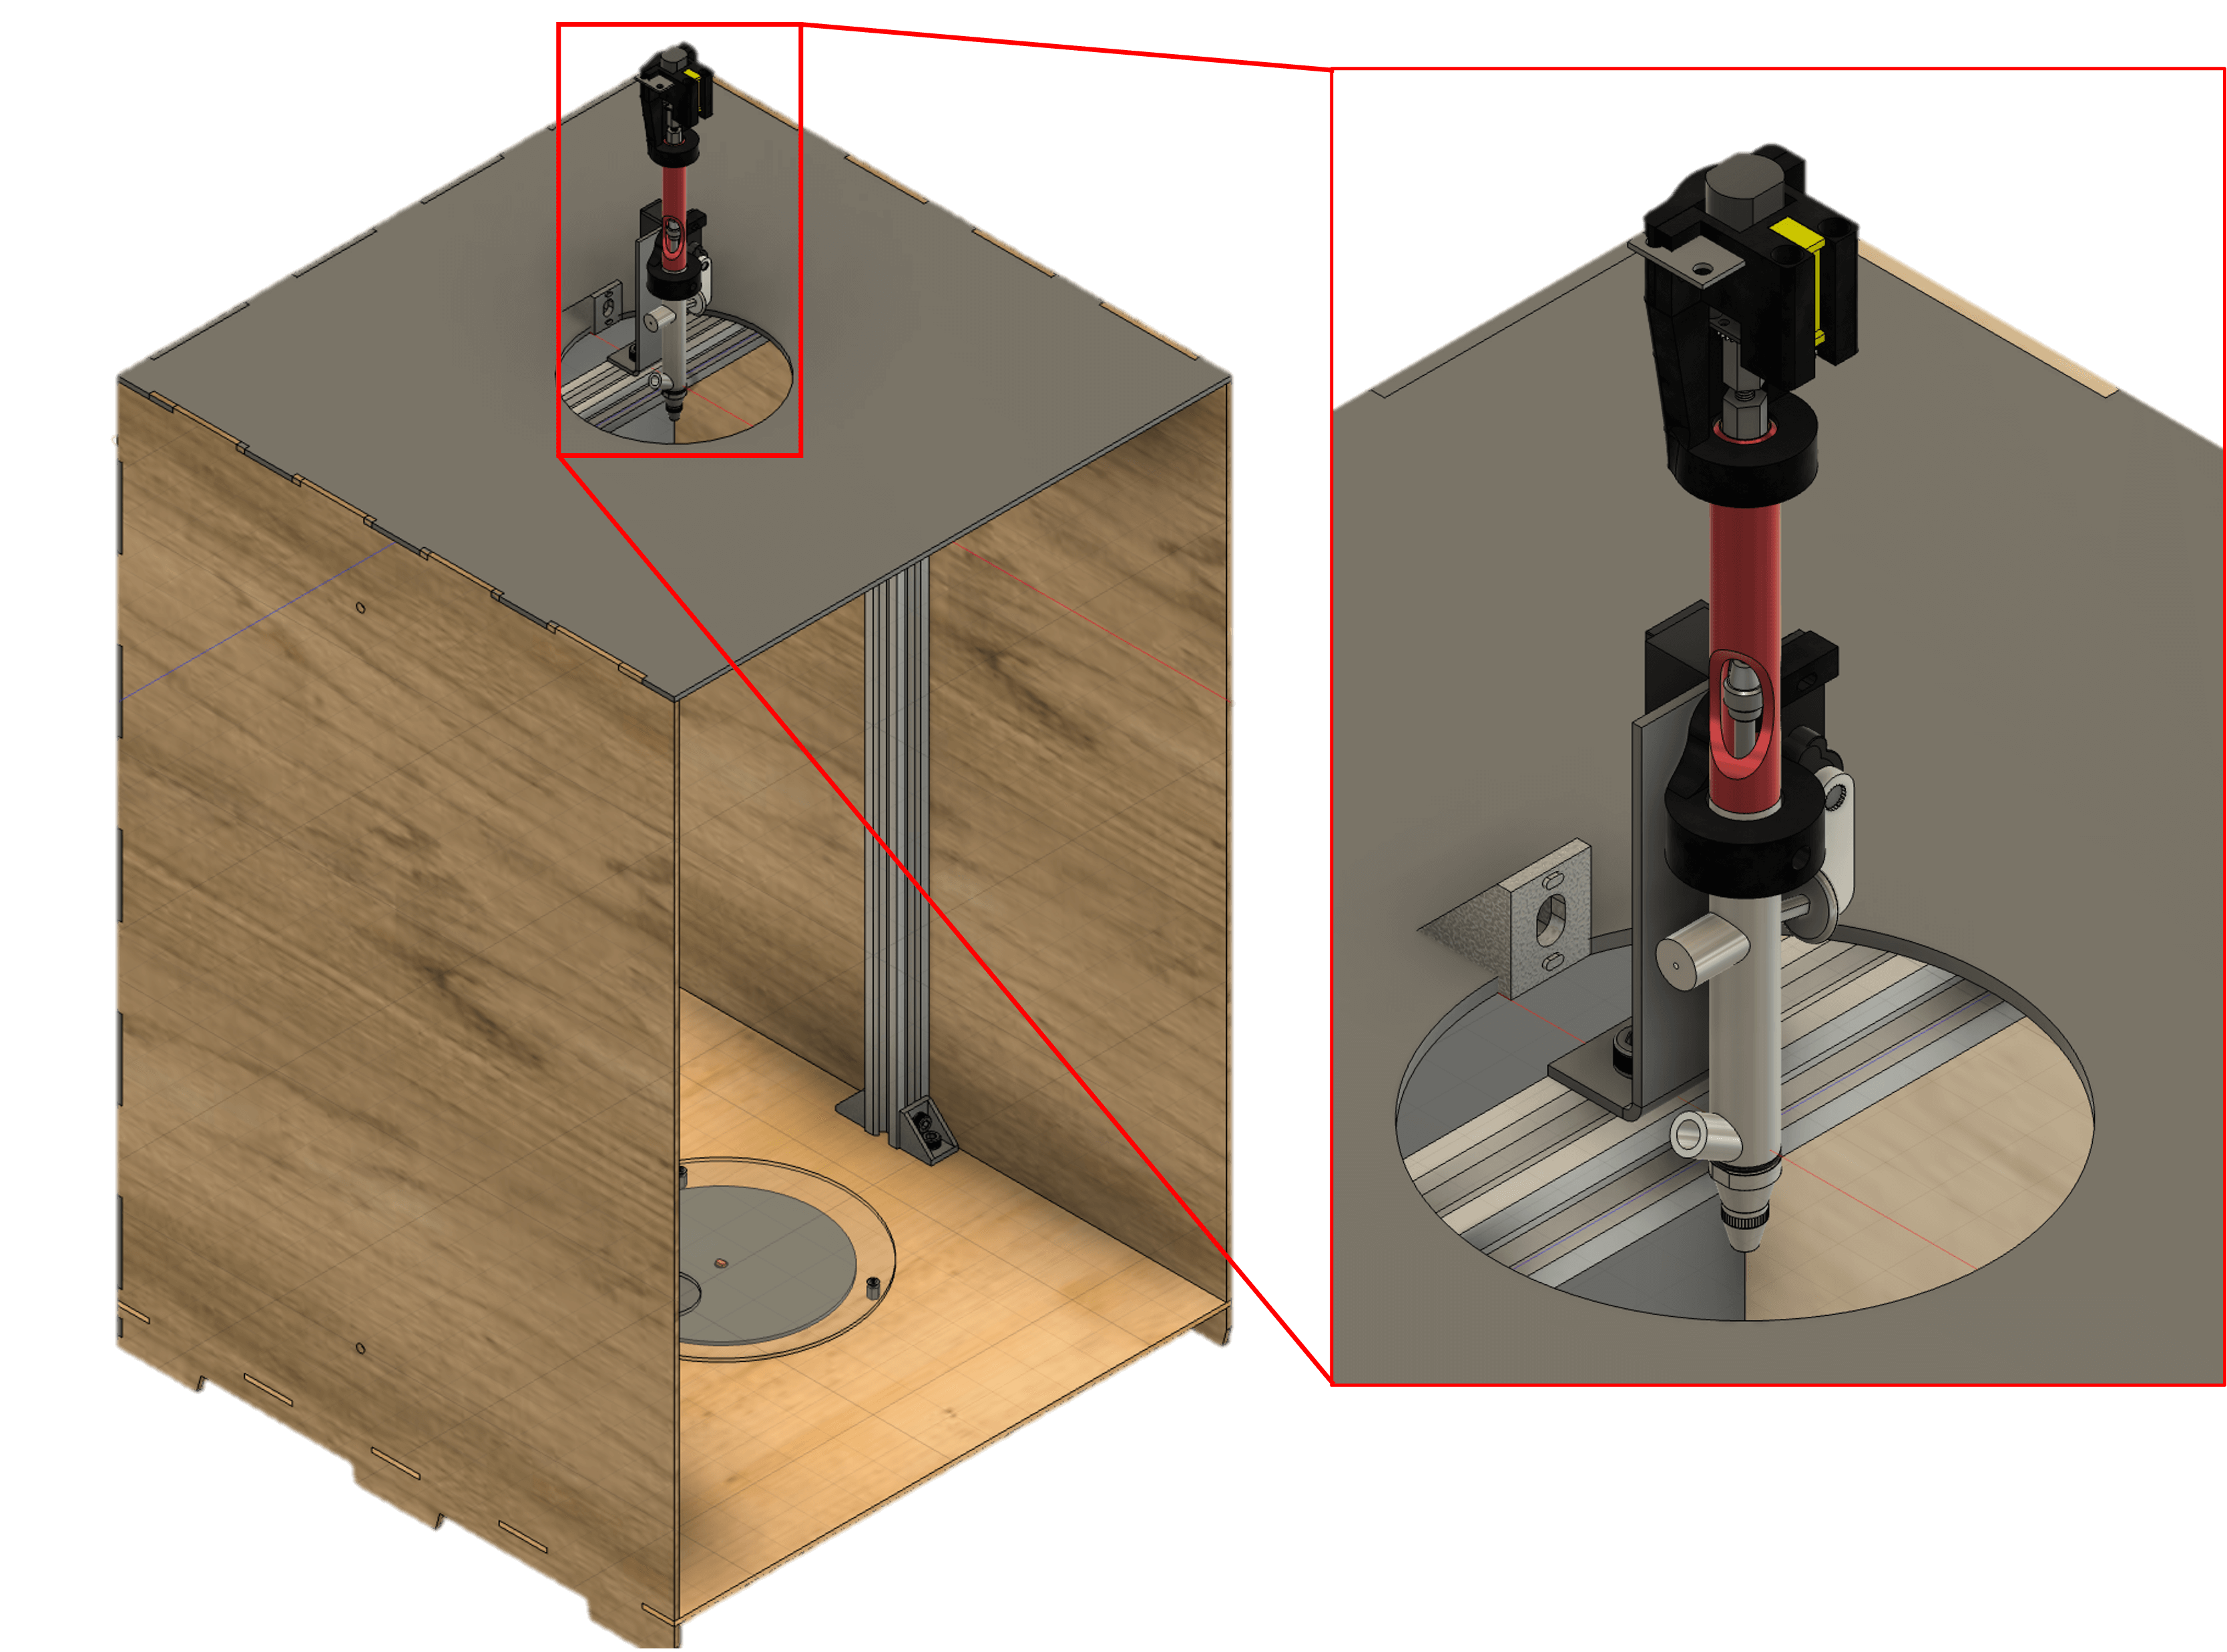
\includegraphics[width = \textwidth]{assets/figures/situation_initiale/machine_initiale.png}
  \caption[Machine originelle]{Machine originelle, avec un zoom sur le système de projection}
  \label{fig:Machine_originale}
\end{figure}

\newpage
La machine de projection se basait sur un aérographe robotisé, où des moteurs géraient les parties mobiles
de l'aérographe qui seraient normalement actionnée à la main :
\begin{figure}[H]
  \centering
  \begin{subfigure}{.35\textwidth}
    \centering
    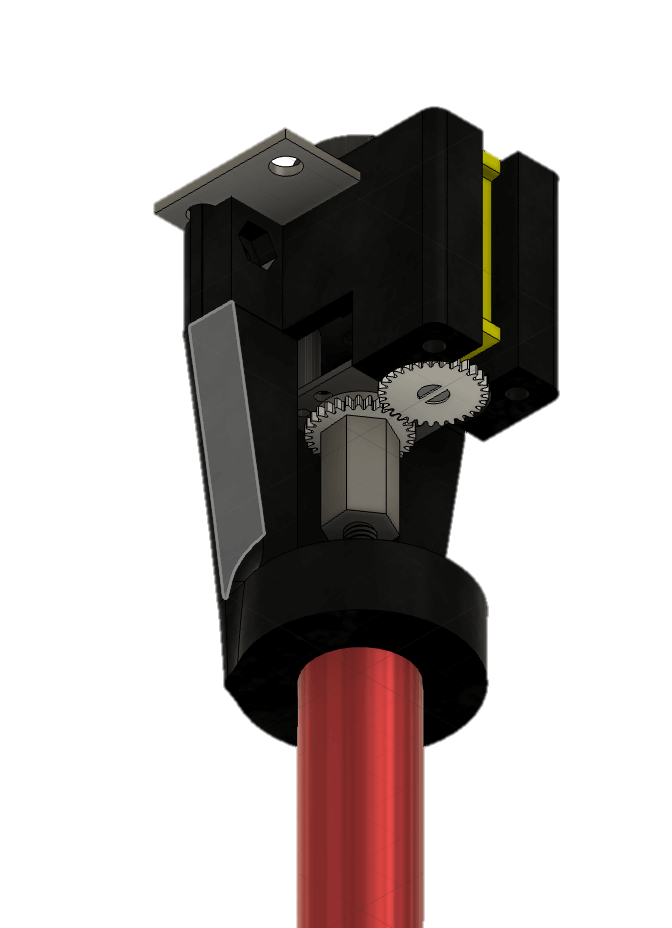
\includegraphics[width=1\linewidth]{assets/figures/situation_initiale/robotisation_aiguille.png}
    \caption{Robotisation de la position de l'aiguille}
    \label{fig:robot_aiguille}
  \end{subfigure}%
  \begin{subfigure}{.65\textwidth}
    \centering
    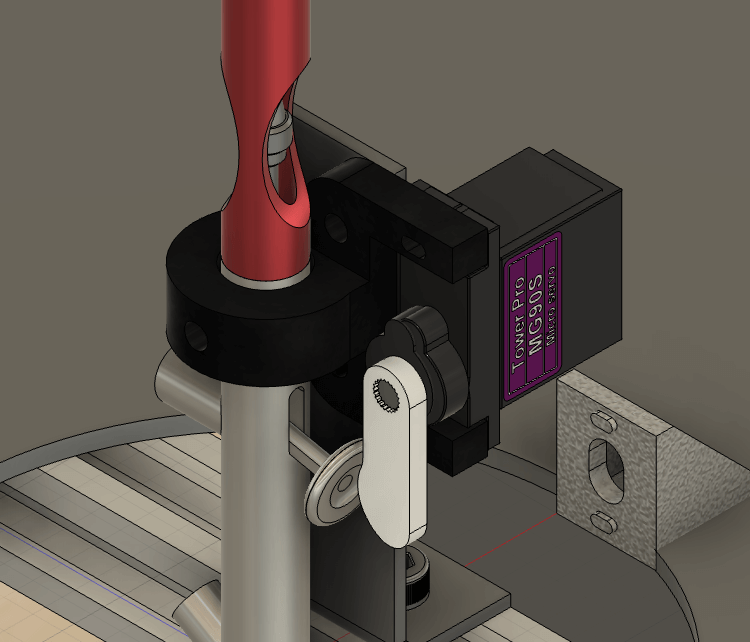
\includegraphics[width=.75\linewidth]{assets/figures/situation_initiale/Robotisation_projection.png}
    \caption{Robotisation du button d'activation du spray}
    \label{fig:robot_spray}
  \end{subfigure}
  \caption{Différentes robotisations de la machine originale}
  \label{fig:robotisations_aerographe}
\end{figure}

Un moteur pas-à-pas de type \textbf{28byj-48}, est situé en bas de l'appareil, ce dernier sert à faire tourner l'écran sur lui même,
c'est donc aussi où l'écran sera disposé lors de sa fabrication:
\begin{figure}[H]
  \centering
  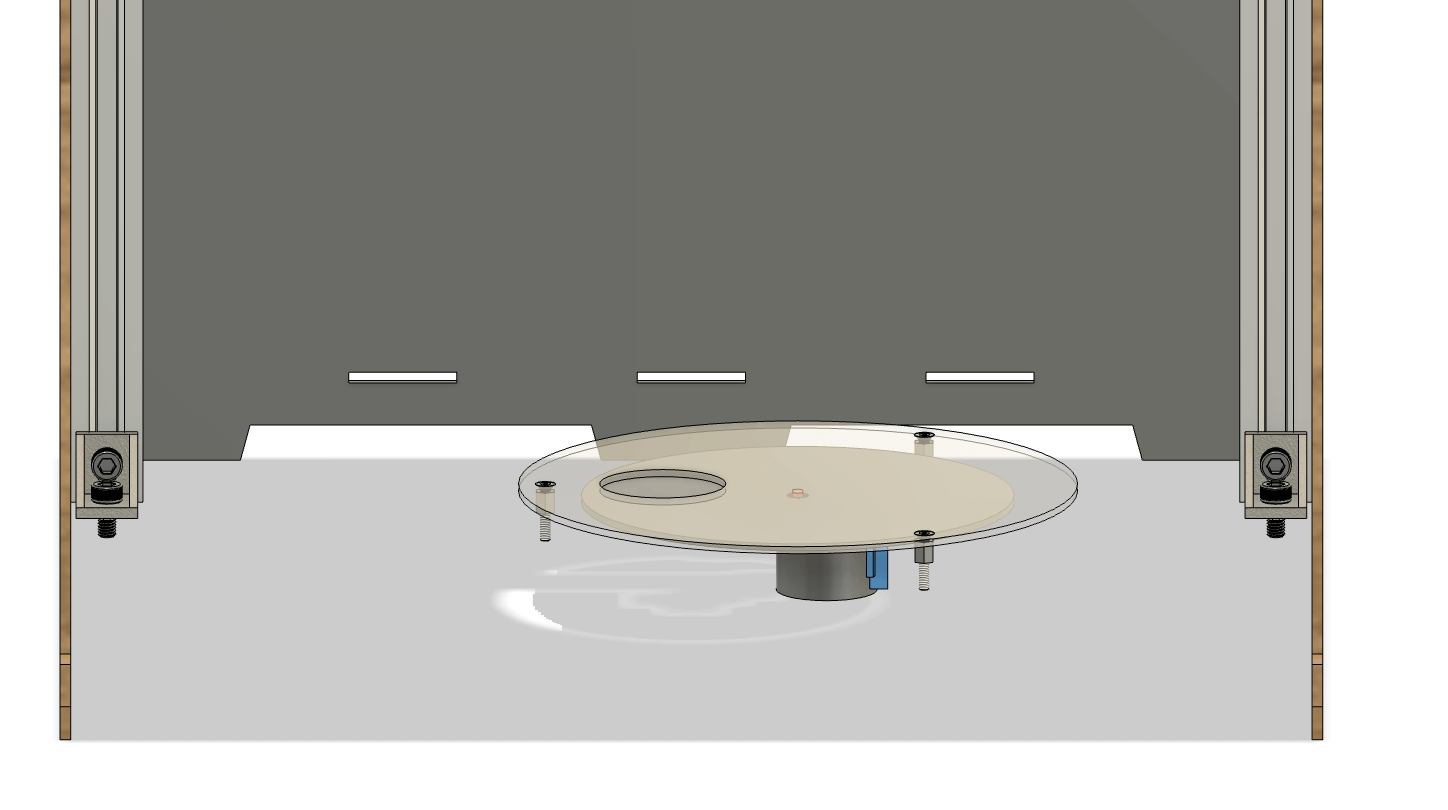
\includegraphics[width = \textwidth]{assets/figures/situation_initiale/rotation_ecran_initiale.png}
  \caption[Rotation écran initiale]{Système de rotation de l'écran}

\end{figure}

\newpage
Tout ces éléments sont contrôlés par un PCB et un arduino nano :
\begin{figure}[H]
  \centering
  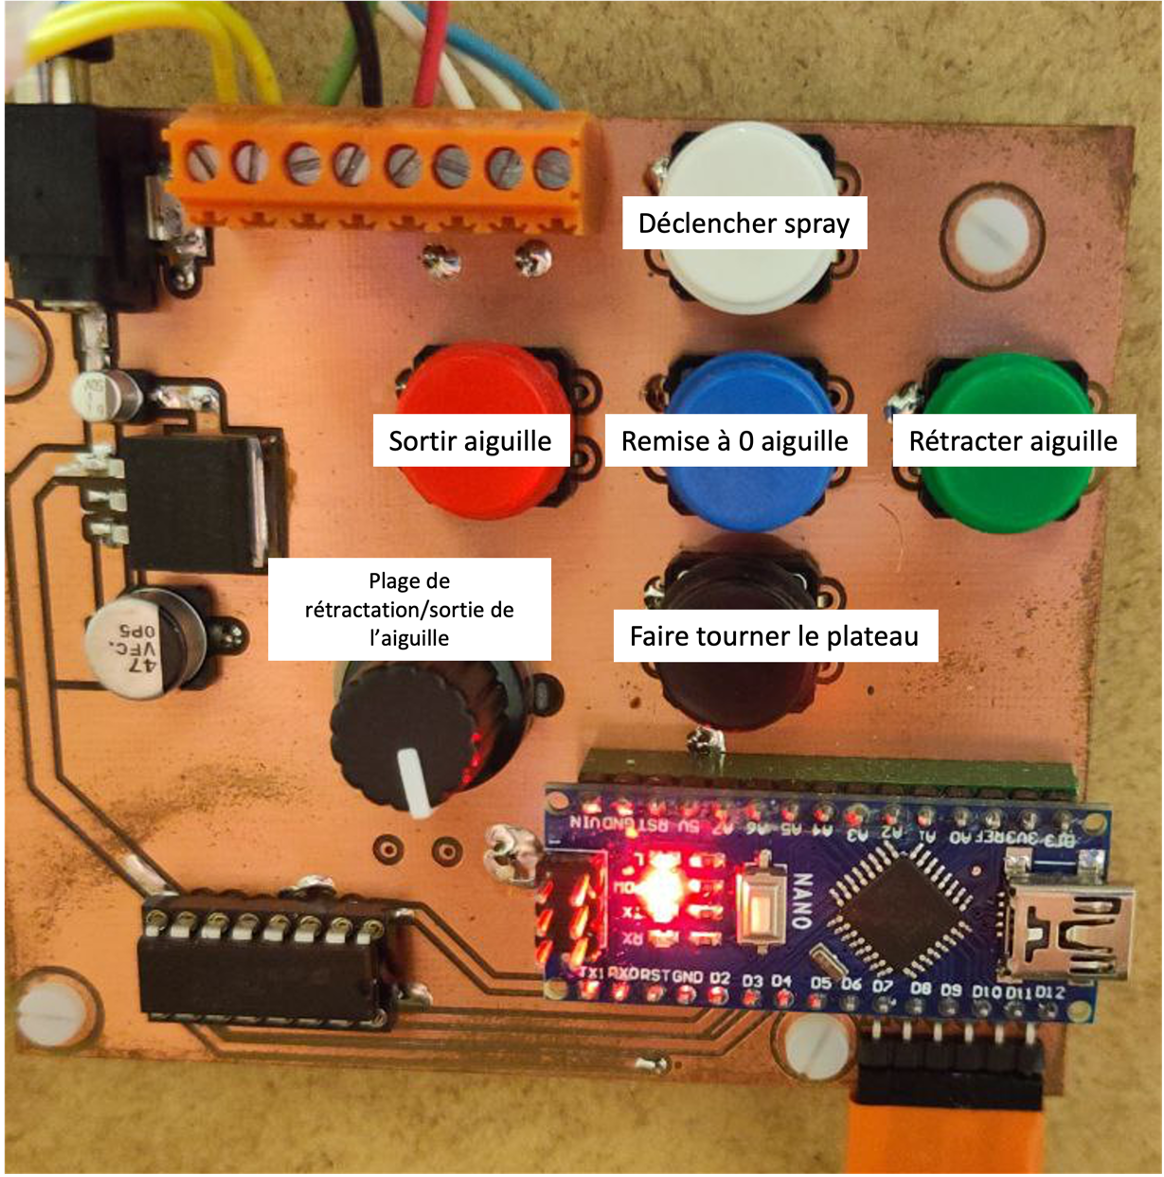
\includegraphics[width = 0.8\textwidth]{assets/figures/situation_initiale/PCB_machine_originale.png}
  \caption[PCB machine initiale]{PCB de la machine initiale et légende de chaque boutons}\label{PCB_machine_initial}
\end{figure}

\section{Problèmes avec la machine}
En effet, la machine d'origine présente plusieurs inconvénients.
\subsection{Aérographe}